\chapter{Classic Bayesian Network Apps}
\label{ch-bnet-apps}

The figures in this chapter were generated using
the free, open source app ``PyAgrum" (see Ref.\cite{pyagrum})\footnote{``agrum" means citric fruit in French. }


Whenever I introduce the subject of Bayesian Networks
to someone who has never met them before, I recommend that the first thing they do is to
download from the internet a ``classic" bnet app  such as PyAgrum\footnote{Alternative choices for bnet apps are Netica by www.norsys.com, or Hugin by www.hugin.com and several others.}, and play with it. It's a sure way of getting hooked
for life. That's how I got hooked, by an early bnet application called Ergo. As you can see from the pictures in this chapter,
the visual output generated by such applications is very ``explainable", intuitive and appealing.

  
In the late 1980's and early 1990's, partially fueled by the invention of
the junction tree algorithm (JTA) (see Chapter \ref{ch-junc-tree}), there occurred much free and commercial software writing activity related to Bnets. Bill Gates was a fan of bnets at that time, and he dedicated a lot of Microsoft manpower to do R\&D of bnets. The first version of Clippy and the first XBox recommender were in fact Bayesian Networks. PyAgrum is a modern version of those ``classic" 1990's apps. It implements many of the same functions (most notably, the JTA) as its predecessors but with a modern Python API and a C++ engine. Other non-classic types of causal AI apps have arisen since the 1990's\footnote{Examples of Causal AI apps of a non-classic type:  Marco Scutari's bnlearn and my JudeasRx, DAG\_Lie\_Detector, Mappa\_Mundi, SCuMpy, SentenceAx, CausalFitBit, texnn.} but PyAgrum fills a big gap in the availability of classic open source bnet apps.\footnote{PyAgrum is similar to my earlier Python app Quantum Fog (QFog). Both implement the JTA, but PyAgrum  has more features and is more polished.
PyAgrum's engine is in C++ and QFog's is in the slower Python.  PyAgrum implements influence diagrams, dynamic bnets
and do-calculus, which QFog doesn't, but QFog implements the JTA for both classical and quantum physics, whereas PyAgrum does no quantum stuff.}

Here are a few of these addictive visuals generated by PyAgrum
for the simple diamond shaped  ``Wet Grass bnet".

To use PyAgrum, one first enters the input data consisting of the structure of the bnet and a TPM (Transition Probability Matrix)\footnote{A TPM is also called
a CPT, which stands for Conditional Probability Table}
for each node of the bnet.


\begin{figure}[h!]
\centering
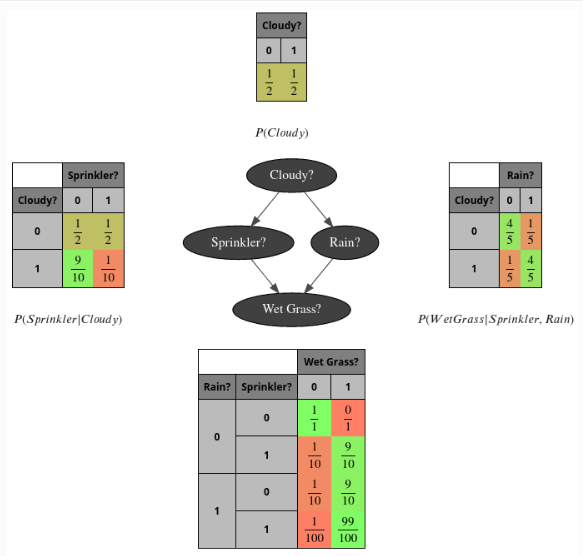
\includegraphics[width=6in]
{bnet-apps/wet-grass-bnet}
\caption{Structure (network, DAG) and a TPM for each node, of the ``Wet Grass" 
bnet.}
\label{fig-wet-grass-bnet}
\end{figure}


\begin{figure}[h!]
\centering
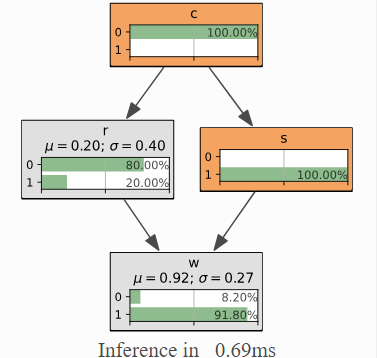
\includegraphics[width=4in]
{bnet-apps/wet-grass-evidence}
\caption{Probability histograms for every node of the Wet Grass bnet,
assuming that as evidence, we observe that $\rvc=Cloudy=1$ and $\rvs=Sprinkler=1$, i.e. the sprinkler was left ON and the day was not cloudy.}
\label{fig-wet-grass-evidence}
\end{figure}

\begin{figure}[h!]
\centering
\includegraphics[width=5in]
{bnet-apps/wet-grass-strength}
\caption{``Wet Grass" bnet drawn so that each arrow's thickness
is proportional to the Mutual Information (a measure of
correlation) between the two nodes connected by the arrow.}
\label{fig-wet-grass-strength}
\end{figure}


When asked to display the input data, PyAgrum shows Fig.\ref{fig-wet-grass-bnet}.



When asked to ``infer" the probabilities of unobserved nodes $\rvr=Rain$
and $\rvw=WetGrass$,
assuming that as evidence, we observe that $\rvc=Cloudy=1$ and $\rvs=Sprinkler=1$, PyAgrum shows Fig.\ref{fig-wet-grass-evidence}.

When asked to redraw the WetGrass DAG so that each arrow's thickness
is proportional to the Mutual Information (a measure of
correlation) between the two nodes connected by the arrow,
PyAgrum shows Fig.\ref{fig-wet-grass-strength}.


PyAgrum can also  

\begin{itemize}

\item consider hard or soft evidence (or no evidence)
for each node. {\bf Hard evidence} means that only
one state of the node is observed whereas {\bf soft
evidence} means that each state of the node occurs with some probability.


\item calculate joint probability distributions and conditional joint probability distributions for multiple nodes of a bnet.
For example, it can calculate  $P(a,b|c,d)$ if $\rva, \rvb, \rvc, \rvd$ 
are 4  distinct nodes of the bnet.


\item find
the most likely value for each node, i.e., find  $x^*.=\argmax_{x.}P(x.)$ where $\rvx.$ contains
 all the nodes of the bnet. $x.^*$ is called the {\bf most probable explanation}.


\item calculate the Markov blanket for any node (See Chapter \ref{ch-mblanket})

\item draw influence diagrams and do associated calculations (see Chapter \ref{ch-influ-diag})

\item calculate conditional probabilities and adjustment formulae  that involve multiple do operators in the condition part. Hence, it does do-calculus (see Chapter \ref{ch-do-calc})

\item do causal DAG discovery (what used to be called structure learning) (see Chapter \ref{ch-struc-learn})

\item calculate dynamic Bayesian networks (see Chapter \ref{ch-dyn-bnets})

\item calculate information theoretic quantities related to a bnet (see Section \ref{sec-def-various-ents})


\end{itemize}
and much more! Numerous examples are included in the 
PyAgrum repo, from The Book of Why (see Ref.\cite{book-why}), Kaggle's Titanic dataset, and other sources.

